\section{Naming}

Naming is a fundamental concept, it allows resources to be bound at different times. Names are bound to objects, this is always relative to a context. One example of this would be path names, e.g. \textit{/usr/bin/emacs}. Name resolution can be seen as a function from context and name to some object. The resolved object can be a context in itself. This gives us a naming network.
\begin{center}
	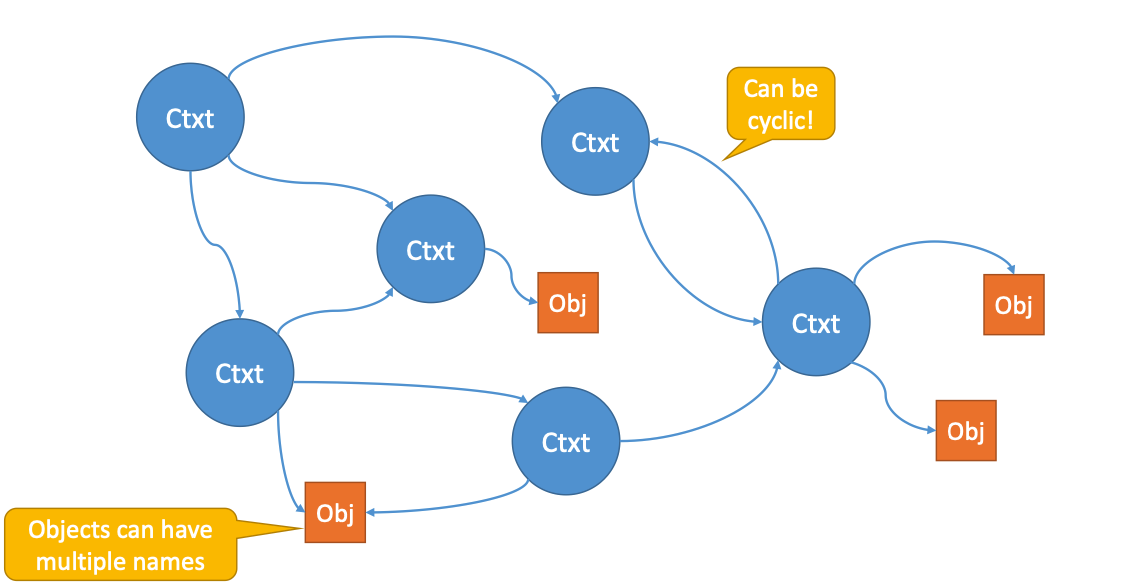
\includegraphics[width=0.8\linewidth]{naming-network.png}
\end{center}

Both synonyms (two names bound to the same object) and homonyms (the same name bound to two different object) can occure.